%===================================== CHAP 2 =================================

\chapter{Basic Theory}

\section{Artificial Neural Networks}

\cite{McCulloch1943} proposes a formal theory for neural functioning, capturing its quintessence within logical propositions. 
The result; artificial neural networks (ANNs), may be trained using feed-forward back-propagation (FFBP), a gradient-descent technique minimizing an error criteria, often based on the \textit{l1}-norm of network output compared to a target output after corresponding input has flowed throughout the network.

\subsection{High-level Outline}
FFBP ANNs may be outlined as follows:
\\
Consider a set of nodes of (artificial) neurons. Each node is connected to a subset of other nodes, together forming a network. Topologically speaking, it is common in traditional approaches to simply construct layers where each node is connected to nodes in the former and preceding layer of the network only (see figure \ref{fig:three_layer_ann}), with distinct weights $\omega$ for every connection. In such an approach, the first layer is the input layer, whereas the last layer is the output layer. Data is then presented to the nodes of the input layer, propagated through the hidden layers by using a transfer function and network weights, before finally arriving at the output nodes. These may represent any functional mapping, such as classification or action selection. Once the input has been propagated throughout the network, i.e. fed forward, the obtained output is matched with a desired output, and an error signal is generated (this can be regarded as the difference between the desired and current output). The error signal is then propagated backwards, the weights being updated to adjust for the error. Note that a learning rate constant, $\alpha$, is usually used to restrain the rate of adjustment in order for a solution to converge.
The transfer function is a function of a node's input, transforming its external input to internal activity. In a sense, the transfer function can be regarded as a crude mathematical approximation to a neuron's internal dynamics, usually providing boundaries for a neuron's possible activation values (representing its membrane potential). Weights may be any real valued numbers, but are usually constrained to a certain interval, for instance the interval [-1, 1]. Some approaches use only binary or tertiary weights, consisting of a set of the weights as for instance \{-1, 0, or 1\}.


\subsection{Formal Outline}
Mathematically speaking, ANNs may be outlined as follows;
\\
a network consists of a set $S$ of $N$ nodes. Furthermore, for every node $i\in S$: $i$ may be connected to a node $j \in S$.
\\
For every such connection, there exists a weight, $\omega_{i,j} \in \Re$, the sub-script denoting a connection weight from node $i$ to node $j$.
\\
A transfer function $f$ is a function $f(\theta)$ of a neuron's total input, $\theta$. A commonly used transfer function is the sigmoid transfer function, simply being 
\begin{equation}\label{sigmoid}
    f(\theta) = \frac{1}{1+e^{-\theta}}
\end{equation}

Neuronal activation $u_j$ of a node $j$ ca be formalised as follows,

\begin{equation}\label{input}
    \theta_j = \sum_{i\in M} u_i \omega_{i,j}
\end{equation}
\begin{equation}\label{activation}
    u_j = f(\theta_j)
\end{equation}
where $M$ is the set of all nodes that have incoming connections to neuron $j$, $M \in S$, and $u_i$ is the activation value of node $i$. This is the principle which is used during the feed-forward phase in an FFBP ANN. In other words, the presented input is propagated throughout the network by calculating activation values for all nodes in the input layer, which then flows through the rest of the nodes in the network in the same manner, until finally arriving at the output nodes.

\begin{figure}
\centering
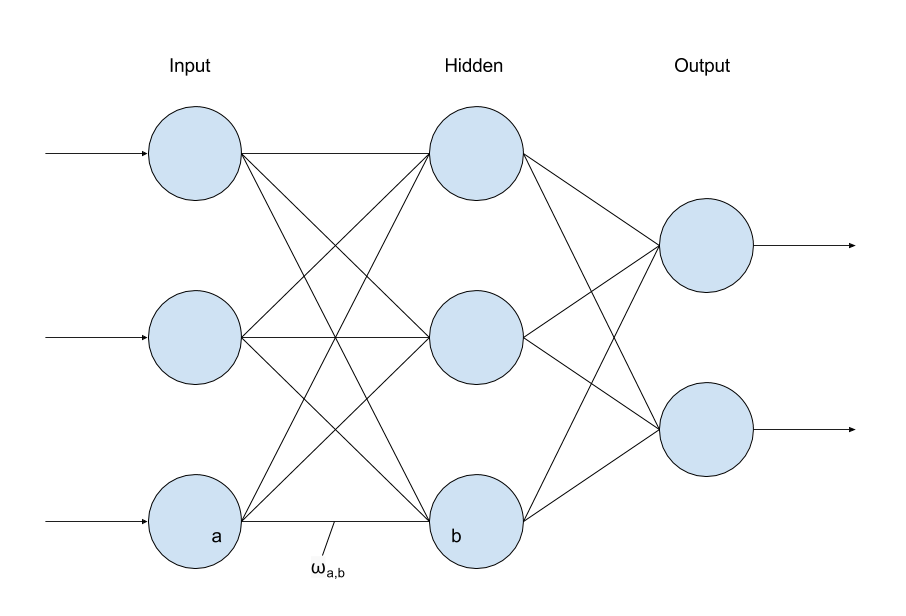
\includegraphics[width=10cm]{fig/three_layer_ann}
\caption{Illustrating a simple three-layer neural network with information flowing from left to right. Every line from one node to another represents a weight $\omega_{i,j}$ connecting two nodes. Note that all nodes are fully connected to each node of the next layer in this example.}
\label{fig:three_layer_ann}
\end{figure}

% ===============================================================================
\subsection{A Trivial Example}\label{trivial_example}

\begin{figure}
\centering
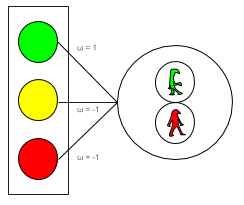
\includegraphics[width=5cm]{fig/trivial_example}
\caption{Illustrating the trivial network topology and weights for the example in \ref{trivial_example}. Note that only one input and one output node would suffice for this type of trivial linear separation.}
\label{fig:trivial_example}
\end{figure}

Consider an example network where the input layer consists of three nodes, see figure \ref{fig:trivial_example} for an illustration. A trivial case is where the input nodes are all binary, for instance symbolising a traffic light with three states; either red, yellow, or green. Thus the input to the network would either be \{1, 0, 0\}, \{0, 1, 0\}, or \{0, 0, 1\}, respectively. These nodes could be connected to nodes in a so called hidden layer, a layer which is neither an input nor an output layer of nodes, which again would be connected to an output layer. For this trivial example, consider that these three nodes are directly connected to the output layer, consisting of one node, which corresponds to an action: Walk or wait. It can fairly easily be seen that a successful action selection can be extracted for weights of {1, -1, -1}, if one interprets the output as walk for positive values, and wait for negative values of output. The transfer function is in this case simply the same as a node's total input $\theta_j$. 
In other events where one would have to perform non-linear separation, several layers of processing may enable a network to perform such non-linear extractions. This would map a non-linear function to a hyperplane in which it is linearly separable. For those acquainted with kernels, the segmentation within neural networks can be compared much to this functional type of hyperplane mapping. Note that it is not the transfer function itself that enables a standard multi-layered ANN to be a universal function approximator - it is the multiple layers of processing. However, the transfer function makes the network differentiable and trainable by gradient-based techniques.


% =====================================================
\section{The Back-propagate Algorithm}\label{BP}

One way of updating the weights in an ANN is by using the back-propagate (BP) algorithm. It is a fairly straight-forward algorithm for searching for optimal weights in an ANN for a particular set of input-output patterns, by minimizing an error-signal which is back-propagated throughout the network. As the generation of an error signal requires an input pattern to be fed forward throughout a network, these two steps are commonly referred to together as feed-forward back-propagation (FFBP). Note, however, that the algorithm does not guarantee convergence towards a global optimum, as it is a gradient-based method, traversing the weight space for a neural network. See figure \ref{fig:steepest_descent} for an illustration of this. An analogy is simulated annealing, which runs the risk of being stuck in a local optimum. However, with just enough 'jiggle', the algorithm may manage to find a better solution, continuing the descent towards a more optimal solution.

Mathematically the back-propagate algorithm requires us to be able to generate a difference for each weight $\omega \in \Omega$, where $\Omega$ is the weight space for the network. Arriving at a given output for a given FFBP ANN through feed-forward propagation using the equations \eqref{sigmoid}, \eqref{input}, \eqref{activation}, one may express the squared error as,

\begin{equation}
    \textbf{E} = \frac{(\textbf{d} - \textbf{o})^2}{2},
\end{equation}
where $\textbf{d}$ is the desired output vector for all output nodes. Dividing by two to account for using two data points in finding the squared error.

This may then be used to calculate a gradient that may be used in updating every weight between the output layer and the preceding layer in the ANN,

\begin{equation}\label{weight_update}
    \omega_{t+1}^{i,j} = \omega_{t}^{i,j} + \Delta \omega_{t}^{i,j},
\end{equation}

In order to perform a weight change in the direction of minimizing the error loss function $\textbf{E}$, the partial derivative of $\textbf{E}$ w.r.t. the weight $\omega_{i,j}$ is used,

\begin{equation}
    \Delta \omega_{i,j} = -\alpha \frac{\partial \textbf{E}}{\partial \omega_{i,j}},
\end{equation}

where $\alpha$ is a learning rate parameter. Note that the sub-script denoting time is dropped for convenience.
The negative is used in order to adjust for the error. Despite the fact that BP does not guarantee convergence towards the global optimum (here minimum), it can be shown that for a sufficiently fine-grained step-parameter (i.e. learning rate), convergence towards a local optimum can be guaranteed. This is due to the nature of the search space, which is continuous and differentiable, but may contain ridges and local minima in terms of the squared error, $\textbf{E}$. However, the smaller the learning rate $\alpha$, the slower the convergence. Another aspect is that for too low an $\alpha$, the gradient's "reach" will also decrease, making it more prone to small stationary points in the weight space. In other words, a learning rate parameter which will converge at a fair rate towards the optimum is preferable. An analogy is that if $\alpha$ is too large, the algorithm is chaotic, resulting in divergence when using gradient descent in weight space. If it is too small, the algorithm is very stable and unable to traverse large parts of the weight space. Lastly, if $\alpha$ is of a preferable size, the algorithm is at the edge of chaos - able to traverse larger parts of the weight space, whilst still converging towards a solution. See figure \ref{fig:steepest_descent} for an illustration of this.

The following derivation is based primarily on the derivation of \cite{Rumelhart1986}, as well as on that of \cite{Russell2009}.
Using the chain rule, one may formally derive $\Delta \omega$ the following way,

\begin{equation}
    \frac{\partial \textbf{E}}{\partial \omega_{i,j}} = \frac{\partial \textbf{E}}{\partial u_j}
    \frac{u_j}{\theta_{j}}
    \frac{\theta_{j}}{\omega_{i,j}},
\end{equation}

the partial derivative w.r.t. the weight between nodes $i$ and $j$ will be cancelled out for all nodes other than $j$. Formally,

\begin{center}
\begin{math}
    \frac{\partial \theta_j}{\partial \omega_{i,j}} = \frac{\partial}{\partial \omega_{i,j}}(\sum_{k \in M}{} \omega_{k,j}o_k),
    \frac{\partial \omega_{k,j}o_k}{\partial \omega_{i,j} = 0 : k \neq i}
    \implies
\end{math}
\end{center}

\begin{equation}\label{delta_theta}
    \frac{\partial \theta_j}{\partial \omega_{i,j}} = u_i.
\end{equation}

\begin{equation}
    \frac{\partial u_j}{\partial \theta_j} = \frac{\partial}{\partial \theta_j} f(\theta_j) = f(\theta_j)(1-f(\theta_j))
\end{equation}

\begin{equation}
    \frac{\partial \textbf{E}}{\partial u_j} = \sum_{l \in L}(\frac{\partial \textbf{E}}{\partial \theta_l} 
    \frac{\partial \theta_l}{\partial u_j})
    = \sum_{l \in L}(\frac{\partial \textbf{E}}{\partial u_l} \frac{\partial u_l}{\partial \theta_l} \omega_{j,l}),
\end{equation}
where $L$ is all nodes to which node $j$ is connected - i.e. the set of nodes with \textit{outgoing} links from $j$. From this it can be seen that when $l$ is an output node,

\begin{center}
\begin{math}
    \frac{\partial \textbf{E}}{\partial u_l} \frac{\partial u_l}{\partial \theta_l} \omega_{j,l} = 
    u_l (u_l - d_l) \omega_{j,l},
\end{math}
\end{center}
Making it possible to obtain the partial derivatives recursively by starting at the output layer and, surprisingly, back-propagating the values into the partial derivatives for $\textbf{E}$ for every weight $\omega_{i,j}$.

In other words, the weight change update in a given layer accounts for the weight change updates of the preceding layers too. Formally,

\begin{equation}\label{recursive_derivative_error_activation_input}
    \frac{\partial \textbf{E}}{\partial u_j}\frac{\partial u_j}{\partial \theta_j} = 
    (\sum_{l \in L}\frac{\textbf{E}}{\partial u_l}\frac{\partial u_l}{\partial \theta_l}) f(\theta_j)(1-f(\theta_j).
\end{equation}

\begin{figure}
\centering
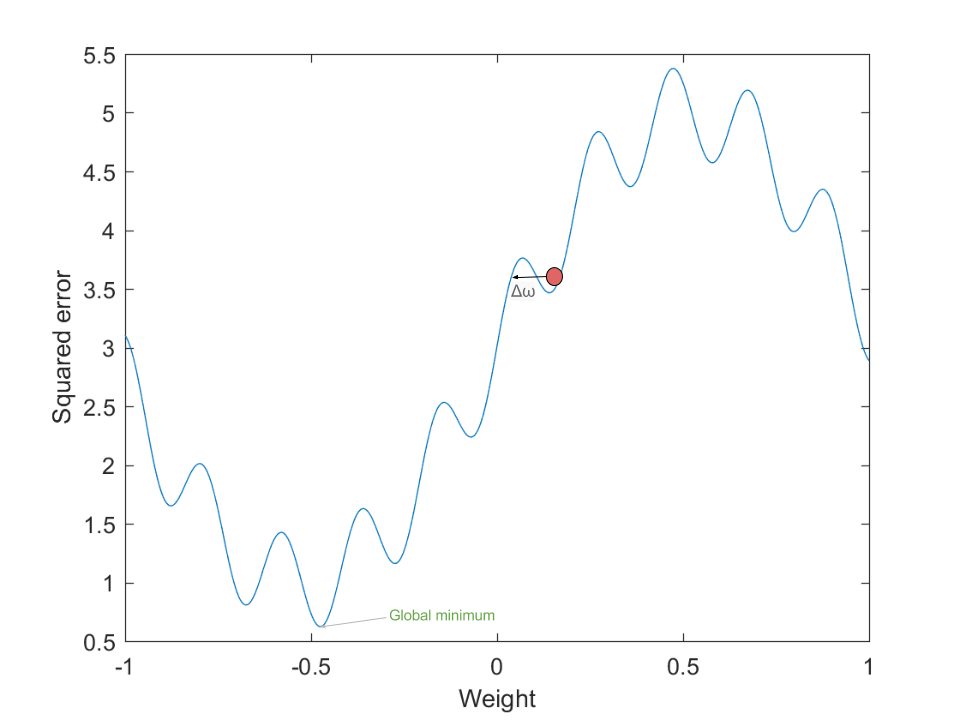
\includegraphics[width=10cm]{fig/error_landscape_with_ball.png}
\caption{Illustrating the error-landscape formed by finding the weights in an ANN that minimize the error. When traversing the landscape formed by $\textbf{E}$, local minima may be encountered (in between ridges). An analogy which is often used in illustrating this is a ball rolling down the hill because of the kinetic energy imposed on it. In this analogy $\alpha$ would be constraining the work of gravity, resulting in smaller or larger velocities, i.e. step sizes $\Delta \omega$ for each iteration of the algorithm.
Too small an acceleration may result in the ball stopping when hitting a small ridge. In the event of this being a local minimum, we would of course prefer for the ball to have enough kinetic energy to traverse the ridge and fall into a lower valley. Therefore, just enough acceleration to traverse the local minima is preferable. However, using too high an acceleration, the ball might not settle into any attractor, possibly the weights will even diverge, the ball being launched into outer space, settling its fate to never again return to the hillside.}
\label{fig:steepest_descent}
\end{figure}

% ====================================
\subsection{Back-propagation Through Time}

The algorithm of section \ref{BP} may be extended by taking into account the $k$ last time-steps of training in a network. Implementations may vary, the key here being a time-dependence. By introducing a measure which averages over the former weights, it turns out that convergence may be faster than when only using BP (as opposed to here BPTT). An alternative approach is to include $k$, or all previous weights, discounting the impact each former weight has exponentially as a function of time.

\begin{center}
\begin{math}
    \omega_{t+1} = \sum_{i=0}^{k}\gamma^i \omega_{t-i},
    \gamma \in (0, 1)
\end{math}
\end{center}


% =================================================================================================
\section{Catastrophic Forgetting}

Catastrophic forgetting \citep{McCloskey1989, Ratcliff1990} is as elaborated on in the introduction (chapter \ref{chpt:intro}) forgetting of model parameters for a domain in which the model has previously been trained. This occurs to such an extent that the performance is equal to that of random weight initialization.

\cite{French1992} addresses the problem of catastrophic forgetting in neural networks that are trained using feed-forward back-propagation, and argues that it occurs because of representational overlap. A method alleviating the problem is to make use of a sparse distributed memory (SDM), which works fairly well until the memory is digested. However, once it is digested severe catastrophic forgetting occurs, and old memories are disrupted in addition to that new ones may not be formed. Furthermore, it is not possible to combine different representations as easily due to the sparsity in an SDM, rendering the approach less generalisable. One way of viewing this is that the distributedness segments more tasks because it acts as a regularizer by constraining the state space. However, this simplification may oversimplify the architecture, causing it to lose out on crucial information due to locally constrained pattern formations. Node sharpening, which is the author's proposed solution, locally constrains input patterns to enhance the most prominent features, effectively resulting in sparse representations. This results in less "noise" being propagated throughout the network, the most principal input nodes being in focus, and a significant reduction in catastrophic forgetting. However, this is done at the cost of attaining a less generalisable model, as node sharpening only looks at the \textit{n} most prominent nodes. Furthermore, today's state-of-the-art algorithms employs different transfer functions, network topologies, and learning. This suggests that the paper's claim, being that that the trade-off between catastrophic forgetting and generalisation is inevitable, may not hold today.

Building on the former work of \cite{French1992}, \cite{French1994} proposes a model which dynamically sharpens the most relevant input nodes. Once two different outputs have been presented to a standard FFBP network, a context bias is calculated in the hidden layer and propagated back to the input layer. Shortly put, this emphasizes the differences of the distinct categories, focusing on segmenting and orthogonalizing on the most prominent properties of difference. Resulting in that more orthogonal, well distributed patterns are learned.
Although this type of segmentation works well, it is still very similar to the former approach of \cite{French1992}, and suffers from the same trade-off between remembering and generalisation. As in other FFBP networks performing gradient descent in weight space \citep{Hinton1989}, the algorithm will only succeed to find the most principal components, scaling with how much information the network is able to store (mainly affected by its size). As a consequence, failing to attain a sufficient accuracy for a given task could be due to ignoring the detailed information present in the segmentation process. Furthermore, it may be the case that only finding the most principal correlations in a distribution does not reveal the distribution's true nature, failing to extract precise correlations and properties. This is at the very core of the sensitivity-stability dilemma \citep{Hebb1949}. One way way of addressing this dilemma is by multi-network systems, which \cite{French1994} suggests in his conclusion. This may produce refined solutions and abstractions and more sophisticated pattern-associations, although seemingly less computationally efficient.


\cleardoublepage